\subsection{Datastructures}

1st iteration:
The idea behind this datastructure, is that by the user only having one vote for each played song, the user is given one reference to track which votes or request. When the lock period of 10 seconds engages at the end of a track, the users reference is locked and cant be changed until next track in queue is playing. When a new track is elected for playing next, all the locked references is added to the according tracks Pscores(Permanent score), by a private function count() encapsulating the pscore, ensuring only the tracks can change it. When a particullar track is played, it's pscores reset to 0. When checking the current standings, the pscore and each reference is accumulated by checking each users reference. If Cpu time is limited on the deployed platform, another implementation would be to keep a list of references to it on each track, this would mean more RAM usage though.
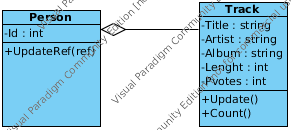
\includegraphics{Images/BackendDSv1.png}